% begin module polar-curve-ex4
\begin{frame}
\begin{example} %[Example 4, p. 677]
What curve is represented by the polar equation $r = 2$?
\begin{columns}[c]
\column{.5\textwidth}

\psset{xunit=0.5cm, yunit=0.5cm, algebraic=true}
\begin{pspicture}(-4.8, -4.8)(4.8,4.8)
\tiny
\psframe*[linecolor=white](-4.8, -4.8)(4.8, 4.8)
%Force a bounding box for pdflatex:
\psline[linecolor=red!1](4.6, 4.6)(4.6001,4.6)
\psline[linecolor=red!1](-4.6, -4.6)(-4.6001,-4.6)%
\fcFullDotBlue{0}{0}%
\psline{->}(0,0)(4.4,0)%
\uncover<3->{%
\rput[bl](1.5, 1.7){\alert<3>{$r=2$}}%
}%
\uncover<3>{%
\parametricplot[linecolor=\fcColorGraph, plotpoints=1000]{-3.14159}{3.14159}{2*cos(t)|2*sin(t) }
}
\uncover<4->{
\parametricplot[plotpoints=1000]{-3.14159}{3.14159}{2*cos(t)|2*sin(t) }
}
\uncover<4->{
\rput[bl](0.6, 0.88){\alert<4>{$r=1$}}
}
\uncover<4>{
\parametricplot[linecolor=\fcColorGraph, plotpoints=1000]{-3.14159}{3.14159}{cos(t)|sin(t)}
}
\uncover<5->{
\parametricplot[plotpoints=1000]{-3.14159}{3.14159}{cos(t)|sin(t)}
}
\uncover<5->{
\rput[bl](3.2, 3.4){\alert<5>{$r=4$}}
}
\uncover<5>{
\parametricplot[linecolor=\fcColorGraph, plotpoints=1000]{-3.14159}{3.14159}{4*cos(t)|4*sin(t)}
}
\end{pspicture}
%\only<handout:0| -2>{%
%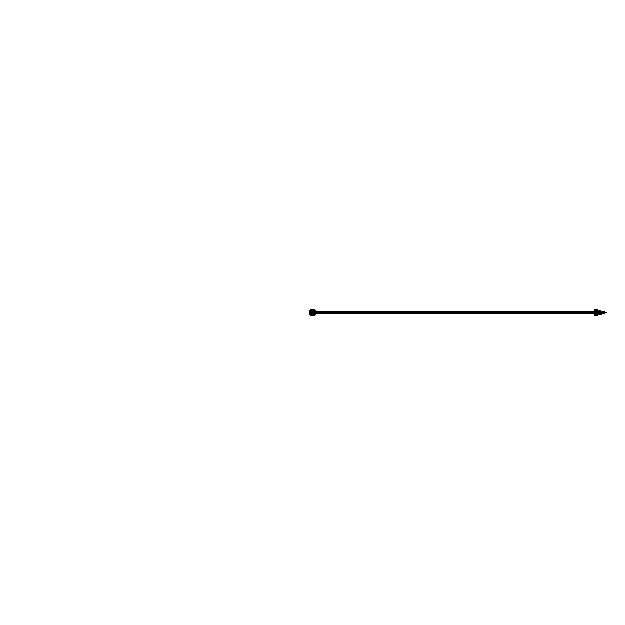
\includegraphics[height=6cm]{polar-curves/pictures/11-03-ex4a.pdf}%
%}%
%\only<handout:0| 3>{%
%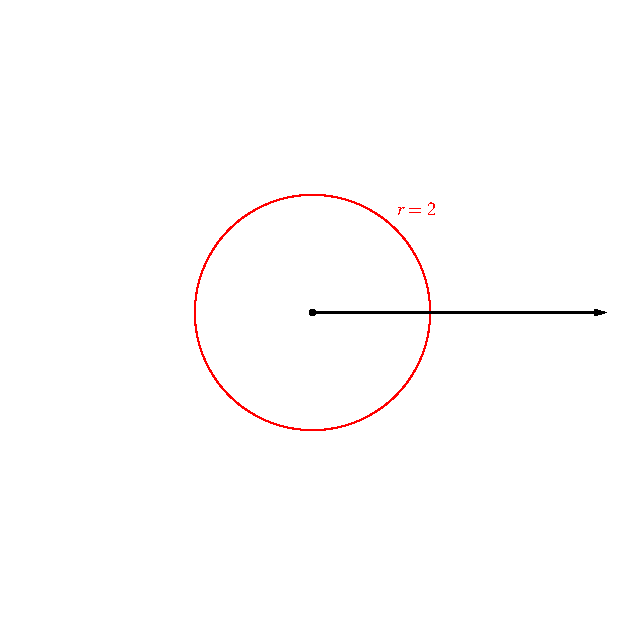
\includegraphics[height=6cm]{polar-curves/pictures/11-03-ex4b.pdf}%
%}%
%\only<handout:0| 4>{%
%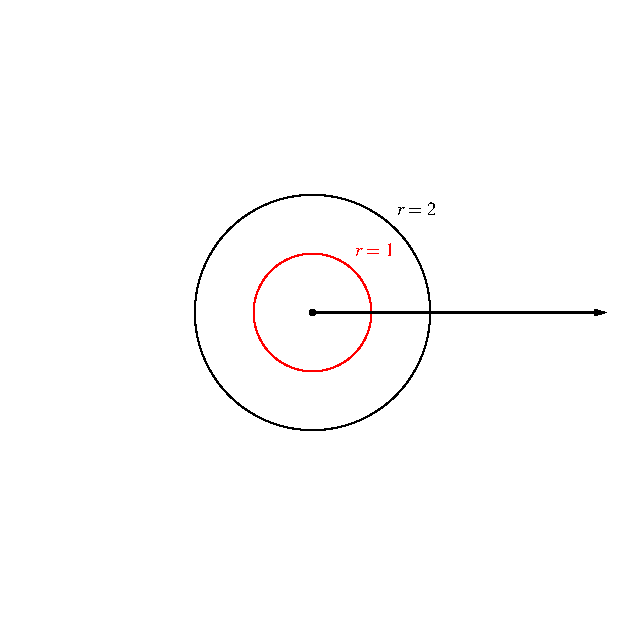
\includegraphics[height=6cm]{polar-curves/pictures/11-03-ex4c.pdf}%
%}%
%\only<5->{%
%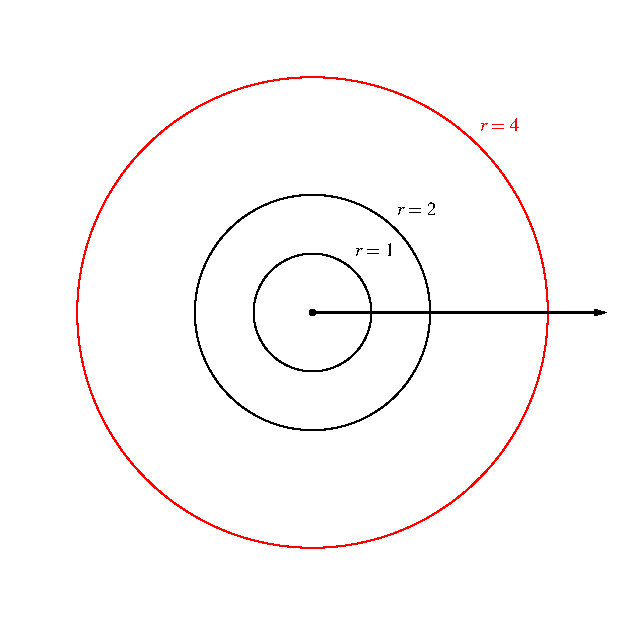
\includegraphics[height=6cm]{polar-curves/pictures/11-03-ex4d.pdf}%
%}%
\column{.5\textwidth}
\begin{itemize}
\item<2->  The equation describes all points that are $2$ units away from $O$.
\item<3->  This is the circle with center $O$ and radius $2$.
\item<4->  The equation $r = 1$ describes the unit circle.
\item<5->  The equation $r = 4$ describes the circle with center $O$ and radius $4$.
\end{itemize}
\end{columns}
\end{example}
\end{frame}
% end module polar-curve-ex4
